%\documentclass[a4paper,12pt]{eskdtext}		%размер бумаги устанавливаем А4, шрифт 12пунктов
\documentclass[a4paper,14pt]{scrartcl}		%размер бумаги устанавливаем А4, шрифт 12пунктов
\usepackage[T2A]{fontenc}
\usepackage[utf8]{inputenc}			%включаем свою кодировку: koi8-r или utf8 в UNIX, cp1251 в Windows
\usepackage[english,russian]{babel}		%используем русский и английский языки с переносами
\usepackage{amssymb,amsfonts,amsmath,mathtext,cite,enumerate,float} %подключаем нужные пакеты расширений
\usepackage[dvips]{graphicx}			%хотим вставлять в диплом рисунки?
\graphicspath{{images/}}			%путь к рисункам

\makeatletter
\renewcommand{\@biblabel}[1]{#1.} 		% Заменяем библиографию с квадратных скобок на точку:
\makeatother

\usepackage{geometry} 				% Меняем поля страницы
\geometry{left=2cm}				% левое поле
\geometry{right=1.5cm}				% правое поле
\geometry{top=1cm}				% верхнее поле
\geometry{bottom=2cm}				% нижнее поле

\renewcommand{\theenumi}{\arabic{enumi}}	% Меняем везде перечисления на цифра.цифра
\renewcommand{\labelenumi}{\arabic{enumi}}	% Меняем везде перечисления на цифра.цифра
\renewcommand{\theenumii}{\arabic{enumii}}	% Меняем везде перечисления на цифра.цифра
\renewcommand{\labelenumii}{\arabic{enumi}.\arabic{enumii}.}% Меняем везде перечисления на цифра.цифра
\renewcommand{\theenumiii}{\arabic{enumiii}}	% Меняем везде перечисления на цифра.цифра
\renewcommand{\labelenumiii}{\arabic{enumi}.\arabic{enumii}.\arabic{enumiii}.}% Меняем везде перечисления на цифра.цифра

\begin{document}
\begin{titlepage}
\newpage

% title page with the name of the university

\begin{center}
\textbf{Федеральное агентство по образованию} \\
\vspace{0.5cm}
\fontsize{10pt}{10.5pt}{\fontseries{b}\selectfont{Государственное образовательное учреждение высшего профессионального образования} }\\
\fontsize{12pt}{12.5pt}{\fontseries{b}\selectfont{“Московский государственный университет приборостроения и информатики”} }\\*
%\hrulefill
\end{center}

\begin{center}
Факультет ИТ  Направление 230105 \\
Кафедра ИТ-6 «Управление и моделирование систем» Квалификация инженер \\
\end{center}

\begin{flushright}
\textit{Утверждаю} \\
Зав. кафедрой \\
\rule{2.9cm}{0.5pt} Мацнев А.П. \\
«\rule{1cm}{0.5pt}»\rule{3cm}{0.5pt} 2010г.
\end{flushright}

\vfill
			% add header

\begin{center}
\textbf{\Large ПОЯСНИТЕЛЬНАЯ ЗАПИСКА \\
к дипломному проекту на тему: }
\end{center}

\vfill\vfill

\begin{center}
\textsc{\textbf{ничо не секу\linebreak ваще}}
\end{center}

\vfill\vfill

\begin{flushleft}
Дипломник \hrulefill Никифоров А.А \\
Группа \hrulefill   шифр \hrulefill \\
Обозначение проекта (работы) \hrulefill \\
\vfill
\textbf{Руководитель проекта (работы) \hrulefill}
\vfill
\begin{center}
Консультанты по разделам:
\end{center}
Наименование разделов: \\
\hrulefill \\
\hrulefill \\
\hrulefill \\
Нормоконтроль \hrulefill \\
\end{flushleft}

\vspace{\fill}

\begin{center}
Москва 2010г.
\end{center}

\end{titlepage}
					% это титульный лист
\tableofcontents 				% это оглавление, которое генерируется автоматически
\part{ТЕХНОЛОГИЧЕСКИЙ РАЗДЕЛ}

\subsection{Модули для GPS микросхемы MAX2769}


\subsubsection{Serial-интерфейс}

\begin{figure}[h]
\center{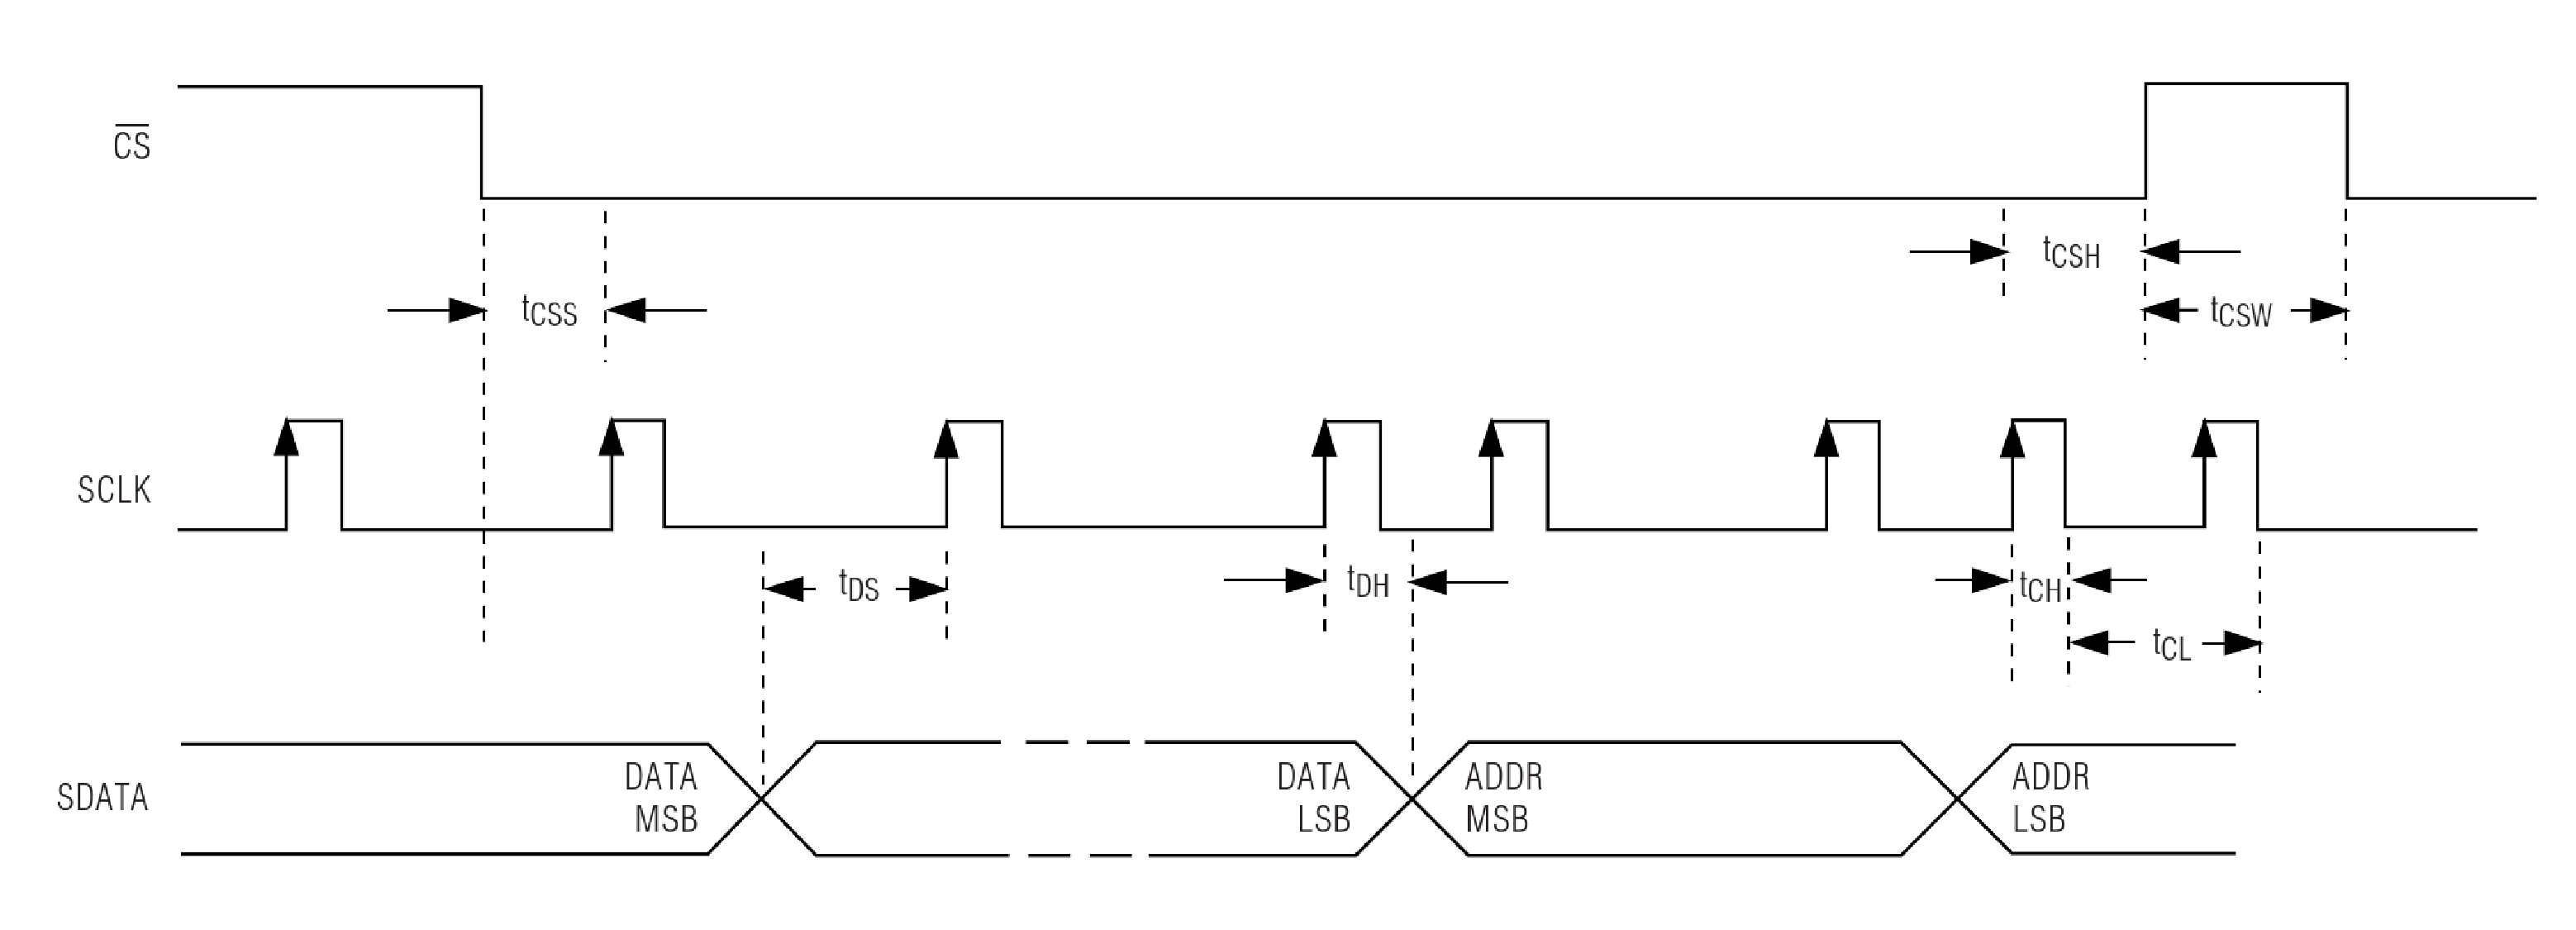
\includegraphics[width=1\linewidth]{./pics/gps_serial_times.eps}}
\caption{Временная диарамма serial-интерфейса GPS}
\end{figure}

\begin{table}[h]
\caption{Таблица 1. Временные требования для serial-интерфейса}
\label{tabular:serial-time}
\begin{tabular}{|c|p{250pt}|c|p{70pt}|}
 \hline  
  Символ & Параметр & Значение & Единица измерения  \\  
 \hline  
  $t_{css}$  & Время между падающим фронтом сигнала $\bar {CS}$ и передним фронтом сигнала SCLK	& 10 & нс  \\  
 \hline  
  $t_{ds}$   & Время установки данных на serial-линию	& 10 & нс \\  
 \hline  
  $t_{dh}$   & Время удержания данных на serial-линии	& 10 & нс \\  
 \hline  
  $t_{ch}$   & Время нахождения Сlock-сигнала serial-интерфейса в состоянии 1 & 25 & нс \\  
 \hline  
  $t_{cl}$   & Время нахождения Сlock-сигнала serial-интерфейса в состоянии 0 & 25 & нс \\  
 \hline  
  $t_{csh}$  & Время между крайним возрастающим фронтом сигнала SCLK и падающим фронтом сигнала $\bar {CS}$ & 10 & нс \\  
 \hline  
  $t_{csw}$  & Время $\bar {CS}$ в активном состоянии    & 1 & такт \\  
 \hline  
\end{tabular}
\end{table}

\begin{figure}[h]
\center{\includegraphics[width=1\linewidth]{./pics/gps_serial_clock_oscylloscope.eps}}
\caption{Clock-сигнал для serial-интерфейса GPS}
\end{figure}

\newpage
					% технологический раздел 
\end{document}
